\documentclass{article}

\title{Internet Video Streaming}
\date{2023-02-28}
\author{Manuel Cadeddu}
\usepackage[italian]{babel}
\usepackage{amsmath}
\usepackage{graphicx}
\usepackage{subcaption}
\usepackage{setspace}
\usepackage{xcolor} 


\begin{document}
	\pagenumbering{arabic}
	\maketitle
	\newpage
	\doublespacing
	\tableofcontents
	\singlespacing
	\newpage

	\section{Segnali Audio e Voce}

		\subsection{Introduzione}
			Un'\textbf{onda acustica} (suono) è una variazione della pressione dell'aria nel tempo. La sua \textbf{ampiezza} è misurata come differenza tra la pressione locale e quella dell'onda sonora. Solo una parte delle onde sonore sono udibili dall'uomo (es. non percepiamo infra/ultra-suoni) e solo una parte di queste è riproducibile tramite le corde vocali (umane).
			\\Come possiamo notare dal seguente grafico, gli umani riescono a sentire suoni con frequenze fino a \textbf{20 KHz} e fino a \textbf{130 dB}. I suoni riproducibili sono di frequenze comprese tra i \textbf{100} e i \textbf{5 KHz} e tra i \textbf{25} e i \textbf{70 dB}. Notare che per musica si intende quella prodotta ad esempio da strumenti.
			\begin{figure}[ht!]
				\centering{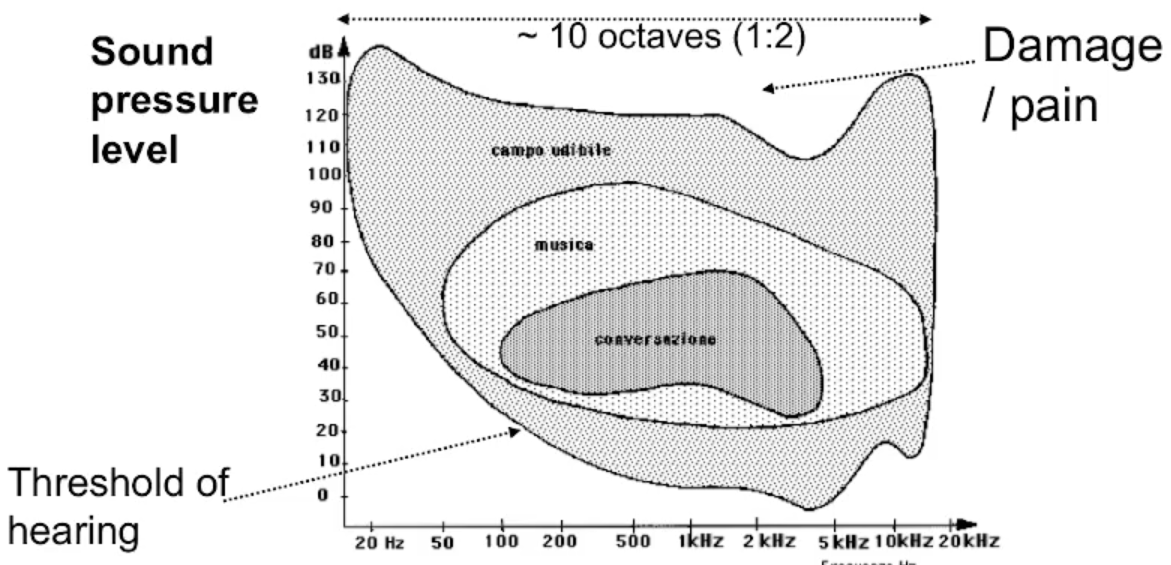
\includegraphics[width=12cm,height=5cm,keepaspectratio]{01_1.png}}
			\end{figure}
			\\I suoni che superano la soglia superiore del Sound Pressure Level (volume del suono, dato dalla variazione di pressione) causano dolore/danni all'orecchio umano, quelli inferiori alla soglia di udibilità invece non sono udibili.
			\\Dal precedente grafico possiamo fare diverse osservazioni:
			\begin{itemize}
				\item le due scale sono logaritmiche (ogni punto equivale ad un "x val" rispetto al precedente): sono udibili suoni con frequenza maggiore fino a 20k volte rispetto alla frequenza minima e suoni con un valore fino a $10^{13}$ volte maggiore del minimo udibile;
				\item \textit{SPL} = $10\log_{10}(P/P_{0})$
				\begin{itemize}
					\item $P_{0}$ è il valore minimo percettibile a 1 KHz
				\end{itemize}
				\item il suono udibile è di circa 10 ottave (raddoppiamento di frequenza);
				\item quando si lavora in dB si hanno sempre misure relative (non assolute).
			\end{itemize}
	
		\newpage
		\subsection{Converione A/D}
			La conversione analogico/digitale consiste nella trasformazione di un segnale continuo in uno discreto. La conversione avviene attraverso diverse fasi:
			\begin{enumerate}
				\item cattura del segnale analogico (es. con microfono);
				\item \textbf{campionamento};
				\item \textbf{quantizzazione}.
			\end{enumerate}

			\subsubsection{Campionamento}
				Il campionamento consiste nella cattura del segnale in precisi istanti di tempo (solitamente ad intervalli regolari). In questo modo si passsa da segnale a tempo continuo a segnale a tempo discreto.
				\begin{figure}[ht!]
					\centering{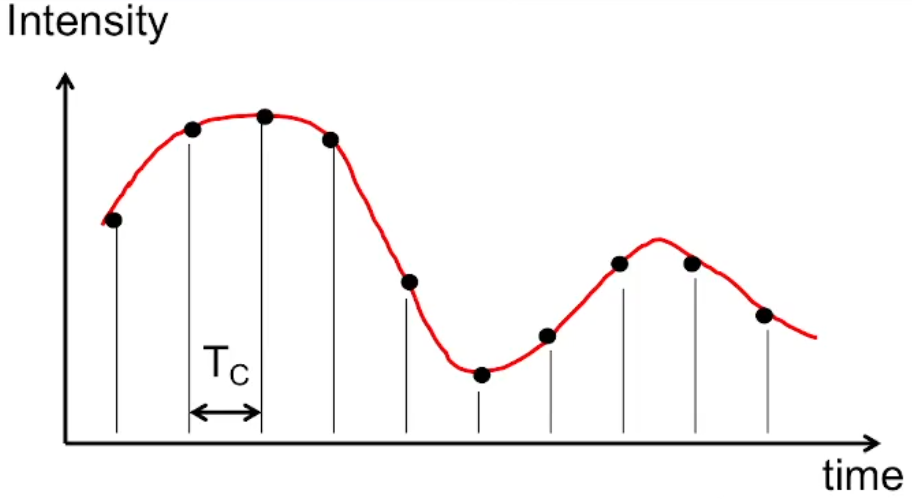
\includegraphics[width=12cm,height=3.5cm,keepaspectratio]{01_2.png}}
				\end{figure}
				\\Nota:
				\begin{itemize}
					\item per poter ricostruire il segnale analogico da quello campionato è necessario che la frequenza di campionamento \textit{$f_{c} = 1/T_{c}$} sia almeno \textit{$2 * f_{max}$} del segnale che deve essere campionato (\textbf{Teorema di Nyquist}).
				\end{itemize}

			\subsubsection{Quantizzazione}	
				La quantizzazione consiste nella mappatura dei valori continui del segnale analogico in valori discreti.
				\begin{figure}[ht!]
					\centering{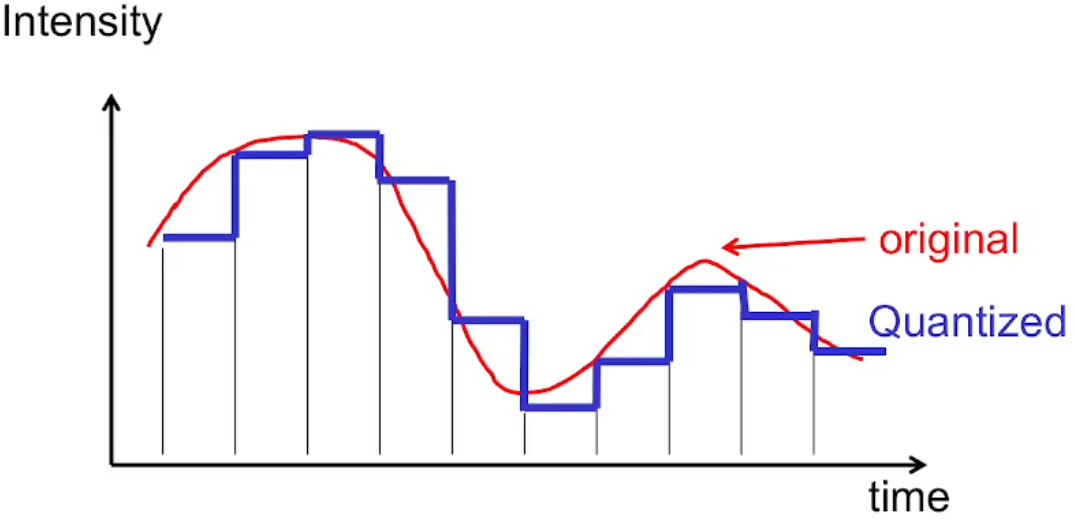
\includegraphics[width=12cm,height=3.5cm,keepaspectratio]{01_3.png}}
				\end{figure}
				\\La tecnica più semplice è la \textbf{quantizzazione uniforme} (o \textbf{lineare}): l'intervallo dei possibili valori viene diviso in intervalli della stessa dimensione.
				\newpage 
				\noindent 
				Notare che spesso viene persa informazione perché si arrotonda il valore del segnale e che, ovunque cada il valore quantizzato, l'accuratezza dell'operazione è sempre la stessa.
				\\Quando si progetta un quantizzatore bisogna fare in modo che il range operativo sia massimo (per catturare "valori estremi") e che la distanza dei livelli di quantizzazione sia minima (per ridurre l'errore di quantizzazione).
				\begin{figure}[ht!]
					\centering{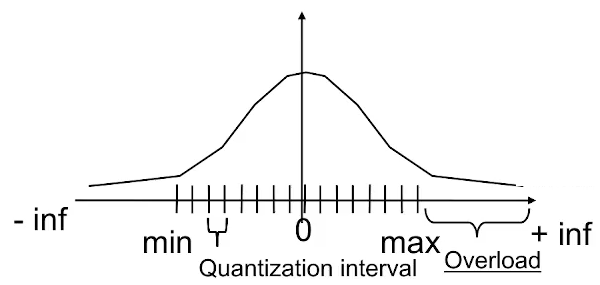
\includegraphics[width=12cm,height=3.5cm,keepaspectratio]{01_5.png}}
				\end{figure}
				\\In caso di \textbf{overload} (il valore del segnale è maggiore del massimo o minore del minimo dell'operational range) il segnale viene associato al valore max o min. Per scegliere la dimensione dell'operational range si usa la seguente regola:
				\begin{center}
					\textbf{operational range} = \textbf{4$\sigma$}
				\end{center}
				
			\subsubsection{PCM (Pulse Code Modulation)}
				Un \textbf{Modulatore a Impulsi Codificati} (PCM) è un dispositivo in grado di campionare il segnale e di quantizzarlo su N bit per campione. Per esempio 12 bit per la telefonia e 16 bit per i CD audio. Maggiore è il numero di bit, maggiore è il \textbf{Rapporto Segnale/Rumore} (\textbf{SNR} = \textbf{Signal-to-Noise Ratio})	e, di conseguenza, il ruomore è meno fastidioso.
				\\Vediamo degli esempi sulla frequenza di campionamento di un PCM lineare:
				\begin{itemize}
					\item CD Audio: 44100 * 16 * 2 = 1,411,200 bit/s
					\begin{itemize}
						\item 44100 = 2 * $f_{max}$;
						\item 16 = bit quantizzazione;
						\item 2 = numero di canali (cassa dx e sx);
					\end{itemize}
					\item Telefono: 8000 * 12 = 96,000 bit/s;
					\begin{itemize}
						\item 8000 = 2 * $f_{max}$ (voce udibile, inoltre la frequenza massima è stata leggermente tagliata);
					\end{itemize}
					\item Video: 720 * 576 * 8 * 30 = 100 Mbit/s;
					\begin{itemize}
						\item 720 * 576 = risoluzione (pixel);
						\item 8 = per colore;
						\item 30 = fps;
					\end{itemize}
				\end{itemize}
				

\end{document}